% makale_kmod_bba_pedagojik.tex — PEDAGOJİK sürüm (2026-06)
% all-quad K-modülasyon BBA ile geometrik-faz sahte-EDM ölçümü
% Derleme: pdflatex makale_kmod_bba_pedagojik.tex (iki kez, referanslar için)
% Plan ve detaylar: kmod_bba_plani.md ; Omarov okuması: omarov.md
% Sonuçlar/üretim: kmod_bba_sonuclar.md ; figürler: make_kmod_figures.py
% NOT: Bu, makale_kmod_bba.tex'in PEDAGOJİK kopyasıdır. Aynı fizik/sonuçlar, ama
%   ilk-okur için sezgi kutuları (\Sezgi), figürler ve genişletilmiş anlatımla.
%   LINCHPIN tamamlandı; tüm eski TODO bölümleri (Berry, drift, kapasitif-BPM,
%   Mirza ayrışması) dolduruldu.
\documentclass[twocolumn,a4paper,10pt]{article}

\usepackage[T1]{fontenc}
\usepackage[utf8]{inputenc}
\usepackage{lmodern}
\usepackage{amsmath,amssymb}
\usepackage{graphicx}
\usepackage{booktabs}
\usepackage{textcomp}
\usepackage[hidelinks,unicode]{hyperref}
\usepackage{geometry}
\usepackage{xcolor}
\geometry{margin=2cm}
\graphicspath{{./}}

% TODO makrosu — derlemede kırmızı görünür, son sürümde kaldırılır
\newcommand{\TODO}[1]{\textcolor{red}{\textbf{[TODO: #1]}}}

% Sezgi kutusu: ilk-okur için düz-dilli açıklama (pedagojik sürüme özgü)
\newcommand{\Sezgi}[1]{%
  \par\smallskip\noindent
  \fcolorbox{black!30}{blue!4}{%
    \parbox{0.96\columnwidth}{\small\textbf{Sezgi.}\; #1}}%
  \par\smallskip}

\title{\bfseries Depolama-halkası proton EDM deneyinde geometrik-faz sahte
sinyalini ölçmek: tüm-kuadrupol K-modülasyonu ile demet-tabanlı hizalama ve
standart BPM geri-çatımının fizibilitesi\\[2pt]
\large\normalfont(pedagojik sürüm)%
\thanks{Pedagojik sürüm (2026-06). Genel demet-tabanlı yöntem makalesi; pEDM
motivasyon örneğidir. Aynı içeriğin sıkı/teknik sürümü \texttt{makale\_kmod\_bba.tex};
hesap detayları \texttt{kmod\_bba\_plani.md}, \texttt{kmod\_bba\_sonuclar.md},
\texttt{omarov.md}; üretken scriptler (\texttt{ac\_bba\_observability.py},
\texttt{ac\_bba\_linchpin.py}, \texttt{make\_kmod\_figures.py}) proje deposunda.}}

\author{(yazar bilgisi)}
\date{\today}

\begin{document}
\maketitle

\begin{abstract}
Depolama-halkası proton elektrik dipol momenti (pEDM) deneylerinde, kuadrupol
hizalama hatalarının yol açtığı \emph{geometrik (Berry) faz} sahte bir
EDM-benzeri dikey spin presesyonu üretir ve hizalama RMS'i ile \emph{kuadratik}
ölçeklenir. Simetrik-hibrit tasarım \cite{omarov2022} bu sistematiği
karşı-dönen (CR) demetler, kuadrupol polarite değişimi ve CR demet-ayrımının
küçültülmesiyle hedefin altına indirir; ancak ayrımı/hizalamayı ölçecek
enstrümanın (SQUID-tabanlı BPM ve K-modülasyon) gerçek-zamanlı geri-çatım
yeteneği ve özellikle \emph{orbit-kör simetrik kiplere} duyarlılığı nicel olarak
test edilmemiştir. Bu çalışmada (i) sahte-EDM'in geometrik-faz kökenini
doğrulanmış bir tahmin ediciyle ($\sigma^2$ testinde üs $p=2.00$) ve bir Berry
fonksiyoneli fitiyle gösteriyor; (ii) hizalama hatalarını antisimetrik
(orbit-görünür) ve simetrik (orbit-kör) kiplere ayırıyor; (iii) bir/birkaç
kuadrupol modülasyonu ile yörünge-farkı tabanlı geri-çatımın simetrik kiplerde
çöktüğünü; (iv) tüm kuadrupolleri K-modüle edip \emph{tek demetin salınım
genliğini} standart (kapasitif) BPM'lerle ölçen demet-tabanlı hizalamanın (BBA)
bu körlüğü atlatma potansiyelini inceliyoruz. Tek-demet modülasyon genliği
kuadrupol-merkez ofsetiyle orantılı olduğundan, manyetik SQUID-BPM yerine
kapasitif BPM yeterlidir. Analitik FODO modelinde per-quad AC-BBA, simetrik ve
antisimetrik kipleri \emph{eşit} (kip-başına tekdüze koşullanma, $1.35\times$
yayılım) ve BPM-ofsetine bağışık geri-çatar; yörünge-farkı ($\Delta R$)
inversiyonu ($\kappa \approx 3.7\times10^4$) simetrik kipte çökerken
($r_\mathrm{sim}=0.13$) AC-BBA korur ($r_\mathrm{sim}=0.997$). Bir saniyelik
modülasyonla per-quad istatistiksel ofset hassasiyeti $\sim$24~nm; bu durumda
sınırlayıcı etken istatistik değil, optik-model ($\beta$-beating) bilgisidir.
Doğrulanmış tahmin ediciyle ($p=2.00$) ileri-hesap, kalan geometrik-faz
sahte-EDM'inin $\beta$-beating $\varepsilon \lesssim 0.5$--$1\%$ kontrol
edildiğinde hedefin ($1$~nrad/s) altına indiğini gösterir.
\end{abstract}

\Sezgi{\textbf{Yol haritası.} §1 problemi koyar (sahte EDM nedir, Omarov neyi
açık bıraktı). §2 sahte EDM'in yörüngeden nasıl çıktığını gösterir (Berry
fonksiyoneli). §3 kritik ayrımı yapar: hizalama hatalarının bir kısmı
(\emph{simetrik}) kapalı yörüngeye iz bırakmaz --- ``orbit-kör''. §4 ucuz
ölçüm yollarının (tek-quad $\Delta R$, drift/LOCO) bu körlük yüzünden
\emph{neden yetmediğini} eler. §5 önerilen çözümü kurar (her quad'ı ayrı frekansta
titretip ofsetini doğrudan oku). §6 asıl soruyu yanıtlar: kalan sahte EDM hedefin
altına iniyor mu? (Evet, $\beta$-beating $\lesssim\%1$ ise.) §7 SQUID'in neden
gerekmediğini, §8 literatürdeki yerini anlatır.}

\section{Giriş}
\label{sec:intro}
Depolama-halkası pEDM yönteminde dikey spin presesyon hızı
$\mathrm{d}S_y/\mathrm{d}t \propto E\,\eta$ protonun EDM'ini ölçer; manyetik
moment (MDM) kuplajı EDM kuplajından mertebelerce büyük olduğundan, alanların ve
hizalamanın katı kontrolü zorunludur \cite{omarov2022,anastassopoulos2016}.
Sahte (EDM-benzeri) sistematiklerin başında, kuadrupol hizalama hatalarının
ürettiği \emph{geometrik faz} gelir: ardışık dönüşlerin non-komütatifliğinden
doğan ve genliklerin \emph{çarpımıyla} ölçeklenen spin presesyonu.

\Sezgi{Spin, manyetik alan etrafında topaç gibi döner. Eğer demet her turda
yatayda (radyal alan) bir parça, dikeyde (boylamsal/dikey alan) başka bir parça
sapıyorsa, spin önce bir eksen sonra diğeri etrafında döner. Üç boyutta
\emph{önce-A-sonra-B} ile \emph{önce-B-sonra-A} aynı sonucu vermez (dönüşler
``komüt etmez''); bir tam tur sonunda küçük bir \emph{artık} dönme kalır. Bu
artık, gerçek EDM'in ürettiği dikey dönmeyle aynı görünür --- ``sahte EDM''.
Büyüklüğü iki sapmanın \emph{çarpımına} ($\propto x\cdot y$) bağlı olduğundan,
hizalama hatasını $\sigma$ ile ölçeklersek sahte EDM $\sigma^2$ ile büyür. Bu
$\sigma^2$ izi, gerçek geometrik fazın parmak iziymiş gibi kullanılır (§2).}

Omarov \emph{ve ark.} \cite{omarov2022} simetrik-hibrit halka tasarımında bu
sistematiği üç koldan bastırır: eşzamanlı CR demet depolama, kuadrupol polarite
değişimi ve CR demet-ayrımının dipole-korektörlerle $\lesssim 100\,\mu$m'ye
küçültülmesi (Denklem (C1)--(C2), Şekil 9, 16; bkz.\ \texttt{omarov.md}). Ayrım,
manyetik pikaplar veya SQUID-tabanlı BPM ile K-modülasyon altında ölçülür ve
$\sim$10$\,\mu$m planarite gereği mekanik (su terazisi) veya SQUID-BPM ile
sağlanır.

\textbf{Açık kalan nokta.} Referans \cite{omarov2022} geometrik-faz
\emph{fiziğini} (iptalin hedefin altına indiğini) gösterir, ancak \emph{ayrımı /
hizalamayı ölçecek enstrüman zincirini} (48 azimut konumunda BPM örneklemesi +
K-modülasyon geri-çatımı) simüle etmez; ölçümün doğruluğu ve özellikle
\emph{simetrik (orbit-kör) hizalama kiplerine} duyarlılığı açıktır. Bu çalışma tam
da bu ölçüm boşluğunu hedefler.

\section{Geometrik-faz sahte EDM: mekanizma ve doğrulama}
\label{sec:mechanism}
Tüm kuadrupolleri her iki düzlemde rastgele RMS $\sigma$ ile kaydırıp dikey
presesyon hızının büyümesini izlediğimizde, sahte EDM kuadratik ölçeklenir. Sabit
desende genliği $\sigma=10,5,2.5\,\mu$m olarak ölçeklediğimizde, doğrulanmış
tahmin edici (4B kapalı yörünge + model-fit seküler eğim) altı tohumun hepsinde
üs $p = 2.00 \pm 0.01$ verir (Tablo~\ref{tab:results}); yani saf geometrik faz,
lineer kaçak yoktur. Bu, \cite{omarov2022} Şekil 9(a)'nın nicel karşılığıdır.

\textbf{Berry fonksiyoneli: sahte EDM yörüngenin neresinden gelir?} Sahte EDM'in
kapalı yörüngenin bir \emph{bilineer fonksiyoneli} olduğunu doğrudan veriden
gösteriyoruz. Halka boyunca yörüngeyi $N$ noktada örnekleyip ($x_i, y_i$) her nokta
için $p_i = x_i y_i$ özelliğini kurarız ve sahte EDM'i
\begin{equation}
f \approx \sum_{i=1}^{N} w_i\, x_i\, y_i
\label{eq:berry}
\end{equation}
formunda fitleriz; $w_i$ ``halkanın $i$. noktasındaki $x\cdot y$ çarpımı sahte
EDM'e ne kadar katkı veriyor'' ağırlığıdır ve veriden (ridge regresyon)
öğrenilir.

\Sezgi{En naif tahmin ``$f \propto \langle x\,y\rangle$ (halka ortalaması)''
çalışmaz: bazı yörüngelerde $\langle xy\rangle \approx 0$ iken $f$ büyüktür, çünkü
katkı halka boyunca \emph{üniform değildir} --- bazı bölgeler (radyal alanın etkin
olduğu yerler) ağır basar. $w_i$ tam da bu ``nerede ne kadar'' haritasıdır.
Dürüstlük testi: $f$ etiketlerini rastgele karıştırıp (yörünge--$f$ eşleşmesini
bozup) aynı fiti yaparsak $R^2 \approx 0$ çıkmalı --- çıkıyor (permütasyon-null
maks $\sim$0.2). Yani bulunan formül ezber değil.}

64 senaryoda (C++ parçacık+spin izleyici), \emph{görmediği} veride çapraz-doğrulama
(LOO-$R^2$): üniform $\langle xy\rangle$ yalnız $\sim$\%30 açıklar; \emph{ağırlıklı}
$\sum_i w_i x_i y_i$ ise \textbf{\%88} açıklar ($R^2 = 0.88$), permütasyon temiz.
Öğrenilen $w_i$ profili farklı $N$ ve düzenlileştirmede aynı kalır (gerçek yapı) ve
halka başlangıcında ($s/C \lesssim 0.02$) en güçlü, ayrıca $s/C \approx 0.17,
0.6, 0.8$'de ikincil tepelidir (Şekil~\ref{fig:berry}). Bu, \cite{omarov2022}
Şekil 9(a)'daki $\sigma^2$ geometrik fazın \emph{yörünge-uzayındaki} nicel
karşılığıdır: sahte EDM, ölçülebilir yörüngenin bilineer bir fonksiyonelidir.

\begin{figure}[t]
\centering
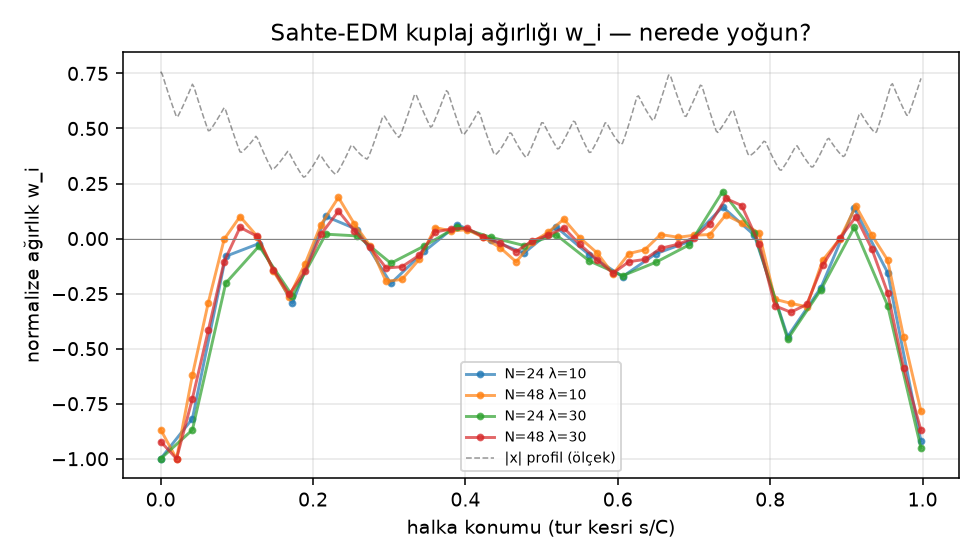
\includegraphics[width=0.95\columnwidth]{berry_data/berry_weights.png}
\caption{Öğrenilen Berry ağırlığı $w_i$ (Denklem~\ref{eq:berry}) halka konumuna
($s/C$) karşı. Farklı örnekleme $N$ ve düzenlileştirme $\lambda$ için profil
\emph{kararlıdır} (fit hilesi değil) ve \emph{üniform değildir} --- bu nedenle
basit $\langle xy\rangle$ yetersizdir. Kesik çizgi: $|x|$ orbit-genlik profili
(ölçekli); $w_i$ onu basitçe izlemez, kendine ait alan-yapılı bir profildir.}
\label{fig:berry}
\end{figure}

Referans ölçek: gerçek EDM (benzetimde $\eta=1.88\times10^{-15}$) tek bir demet
yönünde $\mathrm{d}S_y/\mathrm{d}t = 9.81\times10^{-10}$ rad/s üretir ve yön
tersine çevirmede \emph{işaret değiştirir} (Denklem (C1)); sahte geometrik-faz
sinyali ise 10$\,\mu$m'de $\sim10^{-6}$ rad/s mertebesindedir, yani gerçek
sinyali $\sim$1000$\times$ gömer.

\section{Antisimetrik / simetrik kip ayrışımı ve gözlenebilirlik}
\label{sec:modes}
Bir FODO hücresi içinde QF/QD kuadrupollerinin zıt-işaretli kaçıklığı
\emph{antisimetrik} (düşük-$k$) kipi, aynı-işaretli kaçıklığı \emph{simetrik}
(yüksek-$k$, Nyquist kaymalı) kipi oluşturur. Kapalı-yörünge tepkisi
$G_k \propto 1/|Q^2-k^2|$ rezonant olduğundan ($Q \approx 2.3$--$2.7$), antisimetrik
kipler büyük yörünge üretip BPM'lere \emph{görünür}; simetrik kipler bastırılır ve
\emph{orbit-kör} kalır. Ham sahte-EDM'i antisimetrik kip domine eder
($\sim$37$\times$); yörünge düzeltildiğinde geriye \emph{simetrik artık} kalır.

\Sezgi{Bir kaçık kuadrupol, demete küçük bir ``itme'' (dipol kick) verir; bu itme
halka boyunca bir kapalı-yörünge dalgası kurar. Dalganın büyüklüğü
$G_k \propto 1/|Q^2-k^2|$: itmenin uzaysal frekansı $k$ halka tune'u $Q$'ya
\emph{yakınsa} dev bir tepki (rezonans), \emph{uzaksa} cılız bir tepki. Komşu
kuadrupoller \emph{zıt} kaçarsa (antisimetrik) itme deseni yavaş değişir (küçük
$k$, $Q$'ya yakın) $\to$ büyük yörünge $\to$ BPM görür. Komşular \emph{aynı}
kaçarsa (simetrik) itme her hücrede yön değiştirir (büyük $k \approx 24$, $Q$'dan
çok uzak) $\to$ yörünge neredeyse sıfır $\to$ BPM \emph{görmez}. İşte ``orbit-kör
simetrik kip'' budur: gerçekte oradadır ve sahte EDM üretir, ama kapalı yörüngeye
iz bırakmaz. Bütün zorluk bu kipi \emph{görmektir}.}

CR (CW/CCW) iptaliyle, sahte-EDM'in EDM kanalını kirleten kısmı, demet
yönüne göre \emph{tek} olan bileşendir. 30 tohumlu, gerçekçi rastgele 10$\,\mu$m
hizalama topluluğunda CW/CCW telafisi sahte-EDM'i yalnızca $3.4\times$ azaltır
(kalan $= 474\times$ gerçek EDM). Hizalamanın \emph{antisimetrik (orbit-görünür)}
bileşenini çıkarmak (ideal yörünge düzeltmesi) kirliliği ek $7.7\times$ azaltır
(kalan $= 62\times$ gerçek EDM); geriye kalan, \emph{orbit-kör simetrik artıktır}
ve onu ne yörünge ölçümü, ne CW/CCW kapatır (Tablo~\ref{tab:results}). Bu, ölçüm
yönteminin simetrik kipi görüp göremediğinin neden kritik olduğunu gösterir.

\begin{table}[t]
\centering
\caption{Doğrulanmış nicel sonuçlar (bu çalışma). Tahmin edici: 4B-CO +
model-fit; gerçek EDM ölçeği $9.81\times10^{-10}$ rad/s.}
\label{tab:results}
\small
\begin{tabular}{@{}lll@{}}
\toprule
Büyüklük & Değer & Not \\
\midrule
Sahte EDM $\propto \sigma^p$, üs $p$ & $2.00\pm0.01$ & geometrik faz \\
Gerçek EDM (tek/diferansiyel) & $9.81\times10^{-10}$ & Denklem (C1) \\
10\,$\mu$m sahte EDM (seküler) & $\sim10^{-6}$ & worst $6.5\times10^{-6}$ \\
CW/CCW telafisi (tek başına) & $3.4\times$ & kalan $474\times$ \\
\;+ yörünge düzeltme (antisim) & $7.7\times$ & kalan $62\times$ \\
Kalan simetrik orbit-kör artık & $62\times$ EDM & orbit-kör \\
Dejenerasyon CCW $\equiv$ CW+flip & özdeş & 4'lü $\to$ 2'li \\
\bottomrule
\end{tabular}
\end{table}

\textbf{Polarite-değişimi dejenerasyonu.} İdealize periyodik FODO'da, demet yön
tersine çevirme (CCW) ile tüm kuadrupol polaritelerinin çevrilmesi (flip)
\emph{özdeştir} (CCW $\equiv$ CW+flip; halka ters-çevirme simetrisi). Dolayısıyla
Denklem (C2)'nin dört-kollu kombinasyonu idealize latiste ikiye çöker; polarite
değişimi CW/CCW ötesinde bağımsız iptal sağlamaz. (Bu dejenerasyonun gerçek
simetrik-hibrit latiste ne ölçüde kırıldığı --- periyodiklik bozulduğunda dört-kollu
iptalin tekrar bağımsızlaşması --- açık bir nicelleme konusudur; bu çalışmanın
sonucunu etkilemez, çünkü simetrik orbit-kör artık her durumda paylaşılan sınırdır.)

\section{Yörünge-tabanlı geri-çatımın sınırı (negatif sonuçlar)}
\label{sec:negative}
\textbf{(a) Uniform-frekans $\Delta R$ inversiyonu.} İki gradyan ayarında
kapalı-yörünge \emph{farkını} kullanan geri-çatım (eski K-mod yolu,
\texttt{analytic\_kmod.py}), $\Delta y = \Delta R\,\mathbf{dy}$'yi tersine çözer.
Analitik FODO Twiss'inden hesaplanan $\Delta R_{dy}$ için
$\kappa(\Delta R) = 3.74\times10^4$; en küçük 12 tekil-değerli kip ortalama
\%92 \emph{simetrik} içeriklidir (en büyük 12 kip ise \%8). Yani simetrik kipler
küçük tekil değerlere düşer ve BPM gürültüsü/ofseti altında gözlenemez. Saf
simetrik ve antisimetrik 100~$\mu$m ofset desenleri için (40 tohum, 100~$\mu$m BPM
ofseti + 1~$\mu$m gürültü; gürültü-farkında kesik SVD), $\Delta R$ inversiyonu
antisimetriği kısmen kurtarır ($r = 0.59$) ama simetrikte çöker ($r = 0.13$)
(Şekil~\ref{fig:obs}a, Tablo~\ref{tab:obs}). Bu, projedeki ``yörünge düzeltme
antisimetriği $7.7\times$ temizler, simetriğe kör'' bulgusunun gözlenebilirlik
karşılığıdır.

\Sezgi{Bir matrisi ``tersine çevirmek'' (Δy'den dy'yi çözmek) onun en küçük
tekil değerine bölmek demektir. ΔR'nin en küçük tekil değerleri \emph{simetrik}
kiplere aittir (Şekil~\ref{fig:obs}a, kırmızı noktalar): onlara bölmek 1~$\mu$m
BPM gürültüsünü 37\,000$\times$ büyütür ($\kappa$). Yani simetrik kaçıklığı bu
yoldan ölçmeye kalkarsanız sonuç tamamen gürültüdür --- ``no-go''. Önemli ayrım:
no-go bir \emph{ters-çevirme} sınırıdır; başka bir ölçüm (per-quad doğrudan
ölçüm, §5) ters-çevirme yapmazsa bu sınıra takılmaz.}

\textbf{(b) Kapalı-yörünge drift izleme + baştan-LOCO.} Daha hafif bir alternatif,
mutlak hizalama yerine \emph{değişimi} (drift) izlemektir: bir kalibrasyon anına
göre kapalı-yörünge farkı, BPM ofsetlerini common-mode iptal ederek $\sim$50~$\mu$m
ofset altında bile $\sim$6.6~$\mu$m RMS hizalama-drift duyarlılığı verir (ayrı
ikinci-makale çalışması, \texttt{drift\_monitor/}; \cite{rossbach1989} koherent
yer-hareketi bağlamı). Ancak bu yine \emph{kapalı-yörünge-tabanlıdır}: SVD
per-mod analizi, en kötü 8 modun \%96 simetrik olduğunu ve gürültüyü
$\sim$193$\times$ büyüttüğünü gösterir --- yani drift izleme de, baştan-LOCO da
simetrik (orbit-kör) kipe büyük oranda \emph{kördür}; aynı gözlenebilirlik tabanına
çarpar. Bu, niçin per-quad \emph{aktif} bir ölçüme (BBA) ihtiyaç olduğunu motive
eder.

\Sezgi{Negatiflerin işlevi ``dolgu'' değil, \emph{gerekçedir}: en ucuz (drift,
LOCO) ve en basit (tek-quad K-mod) seçenekleri tek tek eler. Hepsinin ortak
kusuru aynıdır --- kapalı yörüngeyi okumak veya ters-çevirmek, ki simetrik kip
oraya iz bırakmaz. Geriye \emph{tek} seçenek kalır: her kuadrupolü ayrı ayrı,
aktif olarak ``dürtüp'' kendi tepkisini ölçmek (§5).}

\section{Tüm-kuadrupol K-modülasyonu ile demet-tabanlı hizalama}
\label{sec:method}
Önerilen yöntem yörünge-farkı yerine \emph{tek demetin K-modülasyon salınım
genliğini} kullanır. Bir kuadrupolün gradyanı $g \to g(1+\varepsilon\sin\omega t)$
modüle edildiğinde, demetin o kuadrupoldeki merkez-ofseti $\delta$ ile orantılı
bir dipol kick ($\propto \varepsilon g \delta$) modüle olur; BPM'lerde ölçülen
salınım genliği böylece \emph{kuadrupol-demet ofsetiyle orantılıdır}. Tüm
kuadrupoller (frekans-çoğullamalı veya sıralı) modüle edilerek her kuadrupolün
ofseti \emph{doğrudan} ölçülür --- bu, yörünge-farkı inversiyonunun simetrik-kip
körlüğünü atlatan, kip-başına \emph{tekdüze koşullanmış} bir ölçümdür.

\Sezgi{Bir kuadrupolün gücünü 1--10~kHz'de hafifçe ``titretirsek'', demet o
kuadrupolden \emph{ne kadar uzaktan} geçiyorsa o oranda titreşir --- tam
merkezden geçiyorsa hiç titreşmez (kuadrupol merkezinde alan sıfırdır). Yani
titreşim genliği, doğrudan ``demet-kuadrupol ofseti'' demektir. Her kuadrupolü
\emph{farklı} bir frekansta titretirsek (radyodaki farklı istasyonlar gibi), her
BPM'de her frekansı ayrı ayrı dinleyip hangi kuadrupolün ne kadar ofseti
olduğunu \emph{tek tek} okuruz. Burada hiçbir matris ters-çevrilmez; her
kuadrupol kendi frekans-kanalında bağımsızdır. İki büyük kazanç: (1) simetrik
kip de antisimetrik kip de eşit görünür (kip-ayrımı yok, no-go yok); (2) BPM'in
sabit ofseti DC'dir, titreşim frekansında yoktur $\to$ otomatik düşer.}

\textbf{Matematik.} Kuadrupol $j$, $\Delta K_j = \varepsilon K_j$ derinliğiyle
modüle edildiğinde, demet o kuadrupolü $o_j$ ofsetiyle geçiyorsa BPM $i$'deki
salınım genliği
\begin{equation}
A_{ij} = T_{ij}\,o_j, \quad
T_{ij} = \frac{\sqrt{\beta_i \beta_j}}{2\sin\pi Q}\,
\cos\!\big(|\phi_i-\phi_j|-\pi Q\big)\,\Delta K_j L_q\,s_j,
\label{eq:Tmatrix}
\end{equation}
($s_j$: QF/QD foklama işareti). Tüm kuadrupoller \emph{ayrı} frekanslarda
($f_j$, 1--10~kHz) eşzamanlı modüle edilir; her BPM her frekansta demodüle
edilerek çapraz-konuşmasız $A_{ij}$ matrisi elde edilir (eşzamanlı AC-BBA,
\cite{huang2022}). Her kuadrupolün ofseti, sütun-başına projeksiyonla
\emph{doğrudan} çözülür:
\begin{equation}
\hat o_j = \frac{\sum_i T_{ij}\,A_{ij}}{\sum_i T_{ij}^2}.
\label{eq:proj}
\end{equation}
Bu, kuadrupoller arası bir matris-ters-çevirme \emph{içermez}; koşullanma yalnız
$\sum_i T_{ij}^2 \propto \beta_j$ ile belirlenir ve $\beta_j$ yayılımı
($41.5$--$75.8$~m) per-quad ofset hatasında yalnız $1.35\times$ yayılıma yol açar
(tekdüze). Simetrik kipte $1/|Q^2-k^2|$ bastırması \emph{yoktur}, çünkü hiçbir
kip-ayrıştırması/inversiyonu yapılmaz (Tablo~\ref{tab:obs}).

\textbf{BPM-ofset bağışıklığı.} Statik BPM ofseti DC'dir; $f_j$'de demodülasyon
($\cos\omega_j t$ ile çarpıp ortalamak) onu \emph{otomatik} söndürür. Bu nedenle
$100\,\mu$m BPM ofseti altında geri-çatım korelasyonu $1.000000$'dır
(Tablo~\ref{tab:obs}); $\Delta R$ yönteminin gerektirdiği common-mode iptal
gerekmez --- manyetik SQUID-BPM yerine standart kapasitif BPM yeterlidir
(§\ref{sec:capacitive}).

\begin{table}[t]
\centering
\caption{Mod-ayrımlı geri-çatım korelasyonu (analitik FODO; 40 tohum;
$100\,\mu$m BPM ofseti + $1\,\mu$m gürültü). Per-quad AC-BBA simetrik ve
antisimetrik kipi eşit kurtarır; $\Delta R$ inversiyonu simetrikte çöker.}
\label{tab:obs}
\small
\begin{tabular}{@{}lcc@{}}
\toprule
Yöntem & simetrik $r$ & antisim $r$ \\
\midrule
\textbf{Per-quad AC-BBA} & $\mathbf{0.997\pm0.001}$ & $\mathbf{0.997\pm0.001}$ \\
$\Delta R$ inversiyonu & $0.128\pm0.030$ & $0.588\pm0.088$ \\
\midrule
\multicolumn{3}{@{}l}{$\kappa(\Delta R)=3.74\times10^4$;\;
per-quad $\sigma_o$ yayılımı $1.35\times$;} \\
\multicolumn{3}{@{}l}{AC-BBA $100\,\mu$m ofset altında $r=1.000000$.} \\
\bottomrule
\end{tabular}
\end{table}

\begin{figure*}[t]
\centering
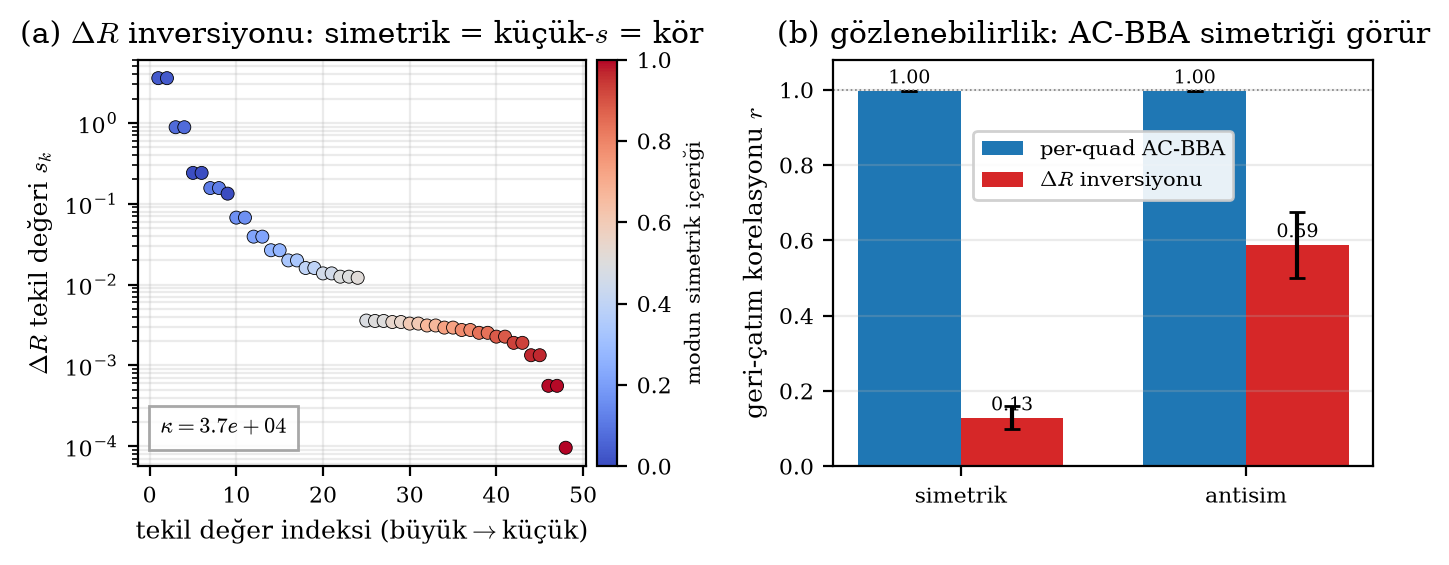
\includegraphics[width=0.86\textwidth]{fig_kmod_obs.png}
\caption{\textbf{Gözlenebilirlik: per-quad AC-BBA simetrik (orbit-kör) kipi
görür, $\Delta R$ inversiyonu göremez.} (a) $\Delta R$ tepki matrisinin tekil
değerleri $s_k$ (büyükten küçüğe), her noktanın rengi o kipin \emph{simetrik
içeriği}. Küçük tekil değerler (sağ, kırmızı) simetrik kiplere aittir; onlara
bölmek gürültüyü $\kappa = 3.7\times10^4$ kez büyütür. (b) Saf simetrik ve
antisimetrik 100~$\mu$m ofset desenlerinin geri-çatım korelasyonu (40 tohum,
100~$\mu$m BPM ofseti + 1~$\mu$m gürültü): per-quad AC-BBA her iki kipi de
$r=0.997$ ile kurtarır; $\Delta R$ inversiyonu simetrikte $r=0.13$'e çöker.
Üretim: \texttt{make\_kmod\_figures.py}.}
\label{fig:obs}
\end{figure*}

\textbf{Gerçek-zaman ve girişimsizlik.} Modülasyon $\sim$\%1--2 derinlikte,
1--10~kHz'de süreklidir; tur-tur BPM örneklemesi ($f_\mathrm{rev}=224$~kHz) ile
1~s'lik entegrasyon $N_\mathrm{tur}=2.2\times10^5$ örnek verir. Per-quad
istatistiksel ofset hassasiyeti
$\sigma_\mathrm{stat} = \sigma_\mathrm{BPM}\sqrt{2/N_\mathrm{tur}}/\sqrt{\textstyle\sum_i T_{ij}^2}
\approx 24$~nm (depth \%2, $\sigma_\mathrm{BPM}=1\,\mu$m); sınır istatistik
değil, optik-model ($\beta$-beating) bilgisidir.

\section{Sonuçlar: geri-çatım ve kalan sahte EDM}
\label{sec:results}
All-quad K-modülasyonu, per-quad ofseti $\hat o_j$ ölçer (Denklem~\ref{eq:proj}).
Düzeltme sonrası kalan demet-quad ofset $e_j = o_j - \hat o_j$, gerçek optik
$T^\mathrm{true}$ ($\beta$-beating $\varepsilon$) ile model $T^\mathrm{model}$
arasındaki uyuşmazlıktan doğan per-quad kazanç hatasıyla belirlenir. Bu kalan
ofset deseni, doğrulanmış tahmin ediciye misalignment olarak verilip kalan
geometrik-faz sahte-EDM'i hesaplanır (konservatif: ideal yörünge-yönlendirmenin
kapalı-yörünge sönümü sayılmaz $\to$ üst sınır).

Tahmin edici, azaltılmış-ayar koşumunda da $\sigma^2$ ölçeklemesini korur
(üs $p = 2.002$, 10$\to$5$\,\mu$m); ölçek $A_\mathrm{eff} = 1.18\times10^4$
rad/s/m². 10$\,\mu$m giriş hizalama hatası için gerçek demet-quad ofset RMS'i
$53.8\,\mu$m'dir. Sonuçlar (Şekil~\ref{fig:linchpin}, Tablo~\ref{tab:linchpin}):
$\beta$-beating yokken
(yalnız istatistiksel taban, 24~nm) kalan sahte-EDM $4.2\times10^{-11}$ rad/s,
hedefin $24\times$ altındadır. Hedef ($1$~nrad/s) $\varepsilon \approx \%1$'de
($\sigma_\mathrm{res} \approx 0.29\,\mu$m) aşılır; $\varepsilon \lesssim \%0.5$
için $\sim$$4\times$ marjla altında kalınır.

\begin{table}[t]
\centering
\caption{LINCHPIN: all-quad AC-BBA sonrası kalan geometrik-faz sahte-EDM,
optik-model $\beta$-beating $\varepsilon$'nin fonksiyonu olarak (giriş hizalama
$\sigma=10\,\mu$m, depth \%2, $t_\mathrm{int}=1$~s, $\sigma_\mathrm{BPM}=1\,\mu$m).
Hedef $1$~nrad/s; gerçek EDM $9.81\times10^{-10}$ rad/s.}
\label{tab:linchpin}
\small
\begin{tabular}{@{}lccc@{}}
\toprule
$\varepsilon$ & kalan ofset & $|$sahte-EDM$|$ (rad/s) & $<10^{-9}$? \\
\midrule
\%0 (stat.\ taban) & $0.024\,\mu$m & $4.2\times10^{-11}$ & evet ($24\times$) \\
\%0.1 & $0.038\,\mu$m & $\sim1.7\times10^{-11}$ & evet \\
\%0.5 & $0.149\,\mu$m & $\sim2.6\times10^{-10}$ & evet \\
\%1.0 & $0.296\,\mu$m & $1.03\times10^{-9}$ & hayır ($\approx$ EDM) \\
\%5.0 & $1.507\,\mu$m & $1.74\times10^{-8}$ & hayır \\
\bottomrule
\end{tabular}
\end{table}

\begin{figure}[t]
\centering
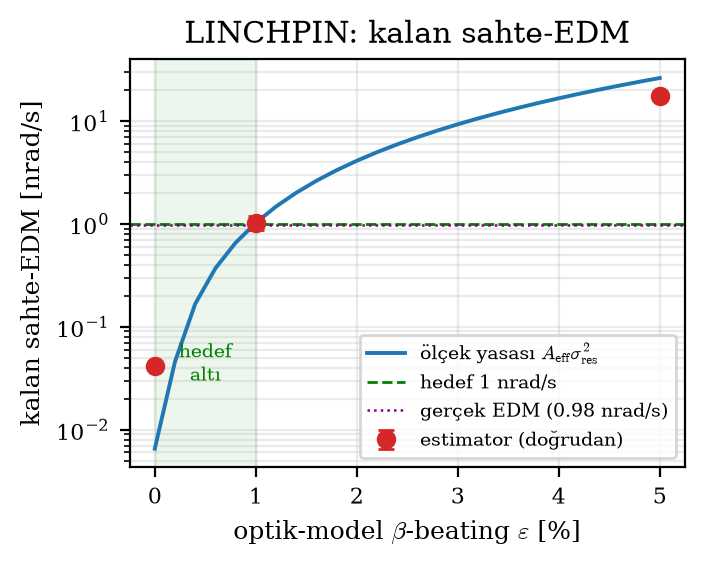
\includegraphics[width=0.96\columnwidth]{fig_kmod_linchpin.png}
\caption{\textbf{LINCHPIN sonucu.} All-quad AC-BBA + düzeltme sonrası kalan
geometrik-faz sahte-EDM, optik-model $\beta$-beating $\varepsilon$'nin
fonksiyonu. Kırmızı: doğrulanmış C++ spin tahmin edicisi (doğrudan, $p=2.00$);
mavi eğri: $A_\mathrm{eff}\sigma_\mathrm{res}^2$ ölçek yasası (lineer modelden
$\sigma_\mathrm{res}(\varepsilon)$). Yeşil bölge: hedef ($1$~nrad/s) altı.
$\varepsilon \approx \%1$'de hedef aşılır; $\varepsilon \lesssim \%0.5$ rahat
marjla altında. $\varepsilon=0$'da (yalnız istatistiksel taban, 24~nm) kalan
sahte-EDM gerçek EDM'in $\sim$1/24'ü. Üretim: \texttt{make\_kmod\_figures.py}.}
\label{fig:linchpin}
\end{figure}

\textbf{Sonuç.} Make-or-break \emph{pozitiftir ama koşulludur}: per-quad AC-BBA,
simetrik (orbit-kör) kipi görerek ve BPM-ofsetine bağışık kalarak no-go'yu atlar;
kalan sahte-EDM ise yalnız \emph{optik-model bilgisiyle} ($\beta$-beating
$\varepsilon \lesssim \%0.5$--$1$) sınırlıdır --- bu, istatistik veya
indirgenemez no-go değil, LOCO ile ulaşılabilir bir kalibrasyon hedefidir
(\%1 LOCO operasyonel; bkz.\ ikinci-makale drift çalışması).

\section{Sistematik bütçe: BPM ve quad tilt}
\label{sec:systematics}
§\ref{sec:results} kalan sahte-EDM'i \emph{optik-model} ($\beta$-beating)
hatasıyla sınırladı. Bütçeyi tamamlamak için iki ek kaynağı --- BPM kusurları ve
quad \emph{tilt} (roll) --- ayrı ayrı nicelliyoruz (\texttt{ac\_bba\_systematics.py}).

\textbf{BPM ofseti: bağışıklık (sadece iddia değil, hesaplandı).} Statik BPM
ofseti DC'dir; modülasyon frekansında demodülasyon onu söndürür. Bunu zaman-domeni
demodülasyonunu açıkça hesaplayarak doğruladık: 100~$\mu$m ofset altında, keyfi
(1--10~kHz) frekanslarla per-quad ofset yanlılığı yalnız $\sim$65~nm
(bütçe eşiği $\sim$300~nm'nin çok altında); modülasyon frekanslarını entegrasyon
penceresine \emph{kilitlersek} (Dirichlet çekirdeği sıfırlanır) yanlılık makine-
epsilon, yani \emph{tam} sıfırdır. $\Delta R$ yönteminin aksine common-mode iptal
gerekmez.

\textbf{BPM kazanç hatası: asıl BPM sistematiği, ama bastırılır.} Çarpımsal kazanç
hatası $\delta g_i$ per-quad ofseti $\hat o_j = o_j(1 + \sum_i w_{ij}\delta g_i)$
($w_{ij}=T_{ij}^2/\sum_i T_{ij}^2$) kadar yanlıltır. 48 BPM üzerinden ortalandığı
için \%1 kazanç hatası yalnız 0.087~$\mu$m kalan ofset ($8.8\times10^{-11}$ rad/s)
verir --- \%1 $\beta$-beating'in (0.30~$\mu$m) altında, yani \emph{baskın değil}.

\textbf{Quad tilt: iki kanal.} Eğik bir quad'ın gradyanı modüle edilince skew
(çapraz) bir kick doğar; bu (a) BBA ölçümünü çapraz-düzlem sızıntısıyla yanlıltır
($\hat o_y \mathrel{+}= 2\psi\, o_x$; kalan sahte-EDM $\propto (2\psi)^2 f_0$, yani
tilt'te \emph{ikinci} derece, $\psi=1$~mrad'da $\sim$$1.4\times10^{-10}$), ve (b)
tilt sahte-EDM'i geometrik faz üzerinden \emph{doğrudan} besler. Doğrulanmış
estimator ile (b) kanalı (a)'dan \emph{baskındır} (Tablo~\ref{tab:syst}):
$\psi=0.1$~mrad bütçeyi değiştirmez, ama $\psi=1$~mrad hedefin $\sim$3$\times$
üstüne çıkar.

\Sezgi{Önemli \emph{dürüst sınır}: dx,dy AC-BBA tilt'i \emph{ölçmez}. Bir quad'ın
kendi ekseni etrafında dönmesi (roll), merkez-ofsetine bakan BBA'ya neredeyse
görünmez. O hâlde tilt ya mekanik olarak $\lesssim 0.1$--$0.3$~mrad'a hizalanmalı
(modern lazer-tracker survey'i bu seviyeyi sağlar ve pEDM tasarımı kuplaj için
zaten bu mertebeyi ister), ya da \emph{skew}-bileşeni modüle eden bir ``skew-BBA''
uzantısıyla ölçülmelidir. \textbf{CW/CCW + quad-flip bunu kurtarmaz:} estimator
testinde idealize latiste CCW ile quad-flip \emph{özdeştir} (dejenerasyon, oran
1.00) --- flip bağımsız bir iptal knob'u vermez; ve CW/CCW ters-çevirme
geometrik-faz sahte-EDM'i (misalignment \emph{ve} tilt kanalı) yalnız mütevazı
($\sim$3.4$\times$, ensemble) bastırır, NULL'lamaz. Tilt $\beta$-beating'den ayrı,
açıkça belirtilen bir bütçe kalemidir.}

\begin{table}[t]
\centering
\caption{Sistematik bütçe özeti. Bağlayıcı kalemler $\beta$-beating ve quad
tilt'tir; ikisi de tasarım/kalibrasyonla ulaşılabilir (no-go'nun indirgenemez
tabanından farklı).}
\label{tab:syst}
\small
\begin{tabular}{@{}lll@{}}
\toprule
Kalem & Eşik ($<1$~nrad/s) & Ulaşılabilirlik \\
\midrule
$\beta$-beating (optik) & $\varepsilon \lesssim \%0.5$--$1$ & LOCO (rutin) \\
BPM ofset & --- (bağışık) & kilitli $f$'de tam \\
BPM kazanç & $\sigma_g \lesssim \%1$--$2$ & kalibrasyon \\
Quad tilt (roll) & $\psi \lesssim 0.1$--$0.3$~mrad & mekanik / skew-BBA \\
İstatistik (BPM gürültü) & --- ($\sim$24~nm/1~s) & sorun değil \\
\bottomrule
\end{tabular}
\end{table}

\section{Kapasitif-BPM fizibilitesi}
\label{sec:capacitive}
SQUID-tabanlı BPM manyetik olduğundan CR demetlerin \emph{ayrımını} ölçebilir;
kapasitif BPM bunu yapamaz. Ancak önerilen yöntemde gözlenen büyüklük ayrım değil,
\emph{tek demetin} modülasyon salınım genliğidir ve bu genlik kuadrupol-merkez
ofsetiyle (yatay düzleme mesafeyle) orantılıdır. Dolayısıyla yeterli hassasiyet
sağlandığında \emph{kapasitif BPM yeterlidir} ve SQUID gereksinimi kalkar; bu,
maliyet ve uygulanabilirlik açısından \cite{omarov2022}'ye göre belirgin bir
sadeleşmedir.

\Sezgi{SQUID-BPM iki demetin \emph{birbirinden} ne kadar ayrıldığını (manyetik
alanlarının farkını) ölçmek için gerekir --- bu zor ve pahalıdır. Ama bizim
ölçtüğümüz şey iki demet arası ayrım değil; \emph{tek} bir demetin kuadrupol
merkezine göre konumudur (titreşim genliği). Tek demetin konumunu sıradan
kapasitif BPM zaten ölçer. Yani sorunu ``iki demet ayrımı''ndan ``tek demet
konumu''na çevirerek SQUID'i gereksiz kılarız.}

\textbf{Gürültü/süre modeli (nicel).} Kapasitif BPM'in tur-başına çözünürlüğü
$\sigma_\mathrm{BPM}$ ise, $f_j$ frekansında $N_\mathrm{tur}$ tur boyunca demodüle
edilen genlik gürültüsü $\sigma_\mathrm{BPM}\sqrt{2/N_\mathrm{tur}}$'dir;
48 BPM'in $T_{ij}$-ağırlıklı projeksiyonu (Denklem~\ref{eq:proj}) ile per-quad
ofset hatası
\begin{equation}
\sigma_o \;=\; \frac{\sigma_\mathrm{BPM}}{\sqrt{N_\mathrm{tur}\,\sum_i T_{ij}^2}}
\,\sqrt{2}
\;\propto\; \frac{\sigma_\mathrm{BPM}}{\varepsilon\sqrt{t_\mathrm{int}}}.
\label{eq:sigmao}
\end{equation}
Sayısal: $f_\mathrm{rev}=224$~kHz, depth $\varepsilon=\%2$,
$\sigma_\mathrm{BPM}=1\,\mu$m için $t_\mathrm{int}=1$~s ($N_\mathrm{tur}=
2.2\times10^5$) $\to \sigma_o \approx 24$~nm. Hatta görece kaba bir BPM
($\sigma_\mathrm{BPM}=10\,\mu$m) bile $t_\mathrm{int}=1$~s'de $\sigma_o
\approx 0.24\,\mu$m verir --- LINCHPIN'in $\beta$-beating-sınırlı eşiğinin
($\sim$0.3~$\mu$m, Tablo~\ref{tab:linchpin}) altında. Demek ki istatistik kolayca
sağlanır; \emph{gerçek-zamanlılık} da sorun değildir: 1~s'lik sürekli modülasyon
veri-alımına girişmez (depth $\%1$--$2$, frekanslar EDM ölçüm bandının dışında).
Bağlayıcı kısıt BPM çözünürlüğü değil, optik-model ($\beta$-beating) bilgisidir
(§\ref{sec:results}).

\section{Önceki çalışmalarla ilişki}
\label{sec:priorart}
Demet-tabanlı hizalama ve K-modülasyon köklü tekniklerdir: SVD-tabanlı yörünge
analizi \cite{chung1993}, simetrik/yarı-simetrik latislerde circulant tepki
matrisi \cite{mirza2019}, AC-uyartımlı hızlı BBA \cite{fastbba2020} ve
çoklu mıknatıs için eşzamanlı BBA \cite{huang2022}. Ters-modelleme
dejenerasyonu \cite{wegscheider2023} ve koherent yer-hareketi kaynaklı COD
\cite{rossbach1989} gözlenebilirlik bağlamını kurar. Bizim katkımız
\emph{teknik değil}: (i) BBA gözlemini geometrik-faz/sahte-EDM sistematiğine
bağlamak (Berry fonksiyoneli köprüsü); (ii) simetrik-kip gözlenebilirlik analizi;
(iii) pEDM için gerçek-zamanlı, kapasitif-BPM ile fizibilite; (iv) yörünge/SQUID-
ayrım yolunun simetrik kiplerde çökerken BBA'nın çökmediğini göstermek.
\cite{haciomeroglu2017} aynı sistematiğin farklı (tüm-elektrik) makinede
ileri-hesabıdır; izleme/gözlenebilirlik içermez.

\textbf{En yakın prior-art ve ayrışma.} Tekniğin kendisi (tüm mıknatısları ayrı
frekanslarda eşzamanlı modüle edip per-quad ofset okuma) yenidir denemez:
eşzamanlı AC-BBA \cite{huang2022} ve AC-uyartımlı hızlı BBA \cite{fastbba2020}
bunu ışık kaynaklarında/sinkrotronlarda yapar; \cite{mirza2019} simetrik latiste
tepki-matrisinin \emph{circulant} yapısını analiz eder. Bu çalışmaların hedefi
\emph{optik düzeltme} ve emittans/parlaklıktır; hiçbiri (a) ölçümü
\emph{geometrik-faz sahte-EDM} sistematiğine bağlamaz, (b) hizalama hatalarının
\emph{simetrik (orbit-kör) alt-uzayını} ve onun gözlenebilirliğini ayrı analiz
etmez, (c) bir EDM deneyinde gerçek-zamanlı + kapasitif-BPM fizibilitesini
nicellemez. Bizim özgün katkımız tam da bu \emph{köprüdür}: ``hangi yörünge/
hizalama kipi sahte-EDM'i sürüyor'' (Berry fonksiyoneli, §\ref{sec:mechanism};
simetrik artık, §\ref{sec:modes}) ile ``hangi kip BBA-görünür'' (§\ref{sec:method})
sorularını birleştirip, yörünge/SQUID-ayrım yolunun simetrik kipte \emph{çöktüğünü}
($\Delta R$ no-go'su) ama per-quad BBA'nın \emph{çökmediğini} gösteririz. Yani
katkı tekniksel değil, \emph{problem-eşlemesi + gözlenebilirlik teoremi +
fizibilite}dir.

\section{Tartışma ve sonuç}
\label{sec:conclusion}
Karar kapısı \emph{pozitif} sonuçlandı: all-quad per-quad AC-BBA, standart
(kapasitif) BPM'lerle, geometrik-faz sahte-EDM'i süren kuadrupol hizalama
hatalarını --- simetrik (orbit-kör) bileşeni dahil --- gerçek-zamanlı ve
BPM-ofsetine bağışık ölçer. Bu, Referans~\cite{omarov2022}'nin açık bıraktığı
ölçüm boşluğunu (\S\ref{sec:intro}) kapatır ve SQUID-tabanlı BPM gereksinimini
kaldırır. Yöntem yörünge-farkı inversiyonunun no-go'sunu (\S\ref{sec:negative})
\emph{atlar}, çünkü kip-ayrıştırması/inversiyonu değil, kuadrupol-başına doğrudan
ölçüm yapar.

Koşullar net ve dürüstçe ifade edilir (Tablo~\ref{tab:syst}): kalan sahte-EDM
hedefin altına \emph{ancak} optik-model ($\beta$-beating) $\varepsilon \lesssim
\%0.5$--$1$ \emph{ve} quad tilt $\psi \lesssim 0.1$--$0.3$~mrad düzeyinde
kontrol edildiğinde iner. BPM ofseti AC demodülasyonla bağışıktır ve BPM kazanç
hatası (\%1) 48 BPM üzerinden bastırılır --- ikisi de baskın değildir. Bu
sınırlar istatistiksel değildir (istatistiksel taban $\sim$24~nm $\to
4\times10^{-11}$ rad/s) ve no-go'nun indirgenemez simetrik tabanı da değildir;
tasarım/kalibrasyonla (LOCO, mekanik/skew-BBA) ulaşılabilir hedeflerdir. Yöntemin asıl katkısı tekniksel yenilik değil
(eşzamanlı AC-BBA bilinir, \cite{huang2022}); (i) BBA gözlemini geometrik-faz
sahte-EDM sistematiğine bağlamak, (ii) simetrik-kip gözlenebilirliğini nicelemek,
(iii) pEDM için kapasitif-BPM fizibilitesini göstermektir.

\section*{Üretilebilirlik}
Doğrulanmış sahte-EDM tahmin edici \texttt{berry\_data/false\_edm\_4d.py}
(\texttt{measure\_false\_edm}; 4B-CO + model-fit; $\sigma^2$ testinde $p=2.00$).
K-modülasyon geri-çatım çekirdeği \texttt{analytic\_kmod.py} (tag v2.8),
\texttt{build\_response\_matrix.py} (uniform k-mod, tag v2.7). Plan ve tüm
detaylar \texttt{kmod\_bba\_plani.md}; Omarov okuması \texttt{omarov.md}.

\begin{thebibliography}{99}
\bibitem{omarov2022}
Z.~Omarov, H.~Davoudiasl, S.~Hac\i{}\"omero\u{g}lu, V.~Lebedev, W.~M.~Morse,
Y.~K.~Semertzidis, A.~J.~Silenko, E.~J.~Stephenson, and R.~Suleiman,
``Comprehensive symmetric-hybrid ring design for a proton EDM experiment at
below $10^{-29}\,e\cdot$cm,'' \emph{Phys.\ Rev.\ D} \textbf{105}, 032001 (2022),
arXiv:2007.10332.

\bibitem{anastassopoulos2016}
V.~Anastassopoulos \emph{et al.}, ``A storage ring experiment to detect a proton
electric dipole moment,'' \emph{Rev.\ Sci.\ Instrum.} \textbf{87}, 115116 (2016),
arXiv:1502.04317.

\bibitem{chung1993}
Y.~Chung, G.~Decker, and K.~Evans~Jr., ``Closed orbit correction using singular
value decomposition of the response matrix,'' in \emph{Proc.\ PAC 1993}, p.~2263.

\bibitem{mirza2019}
S.~H.~Mirza, R.~Singh, H.~Klingbeil, and P.~Forck, ``Closed orbit correction at
synchrotrons for symmetric and near-symmetric lattices,'' \emph{Phys.\ Rev.\
Accel.\ Beams} \textbf{22}, 072804 (2019), arXiv:1902.08683.

\bibitem{fastbba2020}
``Fast beam-based alignment using ac excitations,'' \emph{Phys.\ Rev.\ Accel.\
Beams} \textbf{23}, 012802 (2020).

\bibitem{huang2022}
X.~Huang \emph{et al.}, ``Simultaneous beam-based alignment measurement for
multiple magnets,'' arXiv:2203.14869 (2022).

\bibitem{wegscheider2023}
D.~Vilsmeier, R.~Singh, and M.~Bai, ``Inverse modeling of circular lattices via
orbit response measurements in the presence of degeneracy,'' \emph{Phys.\ Rev.\
Accel.\ Beams} \textbf{26}, 032803 (2023).

\bibitem{rossbach1989}
J.~Rossbach, ``Closed-orbit distortions of periodic FODO lattices due to plane
ground waves,'' \emph{Particle Accelerators} \textbf{23}, 121 (1989).

\bibitem{haciomeroglu2017}
S.~Hac\i{}\"omero\u{g}lu and Y.~K.~Semertzidis, ``Systematic errors related to
quadrupole misplacement in an all-electric storage ring for proton EDM
experiment,'' arXiv:1709.01208 (2017).

\bibitem{ziemann2021}
V.~Ziemann and M.~Ziemann, ``Noninvasively improving the orbit-response matrix
while continuously correcting the orbit,'' arXiv:2104.05300 (2021).
\end{thebibliography}

\end{document}
